Conforme dito no capítulo \ref{chap:mati} o trabalho foi dividido em 4 etapas, nas quais a primeira etapa consistiu no estudo dos DPDs e nos métodos de modelagem deles, a segunda etapa consistiu na implementação desta modelagem em software, que foi optado por utilizar o python, a etapa 3 que consiste na implementação do modelo de DPD escolhido em hardware ultilizando a linguagem VHDL e finalmente na quarta etapa e feita o design do circuito integrado.
Neste capitulo serão exibidos os resultados das etapas 2 já que a etapa 1 consiste no pesquisa bibliográfica e as etapas 3 e 4 serão desenvolvidas na segunda etapa do projeto.

\section{Etapa 2}
A etapa 2 consiste na modelagem do PA em software para posteriormente será feita a modelagem do DPD, e finalmente ser feito o levantamento da quantidade de bits necessários para a implementação do DPD em hardware minimizando os erros de quantização. 
O resultado desse levantamento está presente no gráfico na figura \ref{fig:bits}.
\begin{figure}[ht!]
    \centering
    \captionsetup{justification=centering}
    \caption*{Fonte: Autor}
    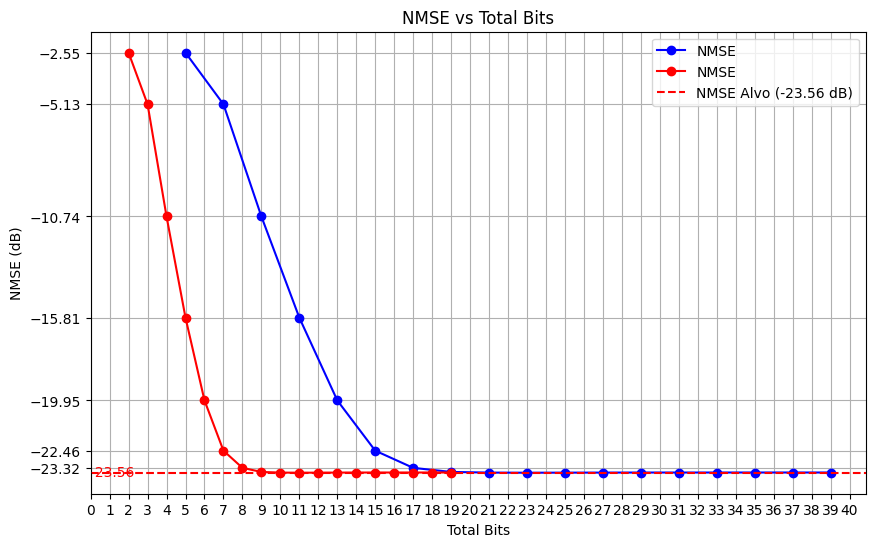
\includegraphics[width=0.5\textwidth]{bits.png}
    \caption{Gráfico Número de bits x NMSE}
    \label{fig:bits}
\end{figure}


Neste gráfico observa-se duas curvas, a curva em azul apresenta a quantidade total de bits total contando com os bits de overflow necessárias para as operações de multiplicação, enquanto a curva em vermelho representa a quantidade de bits de resolução do sinal. Analisando este gráfico observou-se que não existem ganhos significativos no erro a partir de 7 bits, portanto foi feita a modelagem do PA utilizando uma resolução de 8 bits, o resultado alcançado está ilustrado pela figura \ref{fig:modelopa} a seguir.
\begin{figure}[ht!]
    \centering
    \captionsetup{justification=centering}
    \caption*{Fonte: Autor}
    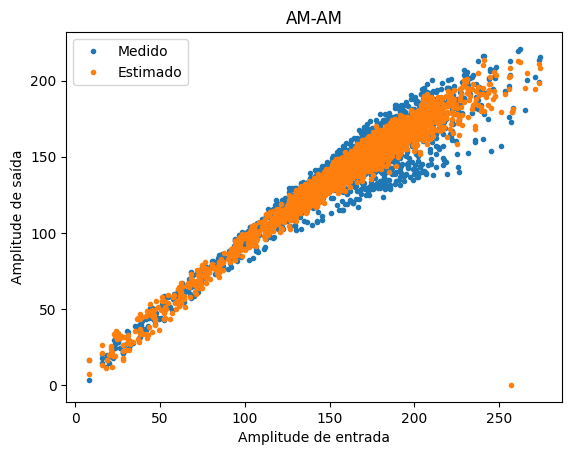
\includegraphics[width=0.75\textwidth]{modeloPA.png}
    \caption{Modelo do PA em vírgula fixa}
    \label{fig:modelopa}
\end{figure}

Verificando a figura \ref{fig:modelopa}, observa-se que o modelo apresentou o resultado esperado e partir disso foi feita a modelagem do DPD, cujo resultado está ilustrado pela figura \ref{fig:modelodpd} a seguir

\begin{figure}[ht!]
    \centering
    \captionsetup{justification=centering}
    \caption*{Fonte: Autor}
    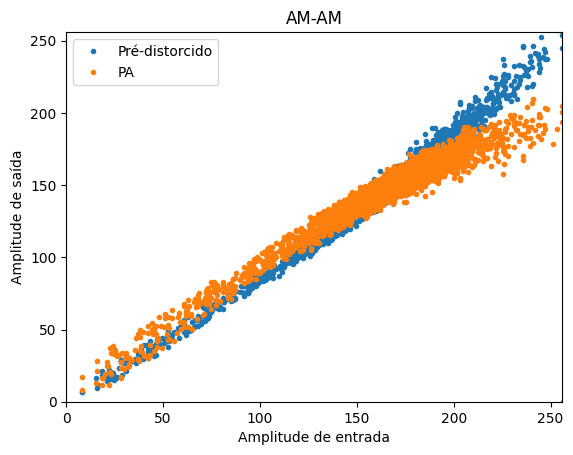
\includegraphics[width=0.75\textwidth]{modelodpd.png}
    \caption{Modelo do DPD em vírgula fixa}
    \label{fig:modelodpd}
\end{figure}